\documentclass[11pt]{article}
\usepackage{graphicx}
\usepackage{hyperref}
\setlength{\parindent}{0pt}
\begin{document}
\title{School of Computer Science and Statistics \vspace{0.3cm}\\Trinity College Dublin\vspace{0.7cm}\\
\includegraphics[scale=1.5]{TCD.jpg}\vspace{0.8cm}\\Final Report\vspace{0.3cm}\\CS7038: Group Project}
\author{Yafie Qu, Hao Guan, Jeremiah Dunn, Saloni Sharma}
\maketitle
\section{Overview of the Project}
\subsection{Story}
Our game takes place on a spaceship which is on a long journey. The ship's computer begins malfunctioning, different subsystems start failing and the security system begins to malfunction. The crew of the ship is in stasis and unaware of the situation. The player  character, the maintenance droid is the only unaffected robot or computer on the ship. His task is to restore power to ship's subsystem while avoiding the security system. The ship's fate is in the hands of this humble maintenance droid.
\subsection{Theme}
This is the International Year of Light and Light-based Technologies. This is a United Nations observance that aims to raise awareness of the achievements of light science and its applications and importance.\\

Our game incorporates light as one of the main mechanics for exploring the ship. When the space ship is wrecked and malfunctions, it looses all its power sources and light. The player character returns power to the ship, gradually lighting it up in the process. Restoring light makes the ship easier to navigate and directs the player towards the exit of each level.\\

\subsection{Initial Design}
The game is an exploration based 2D platformer similar to games like \textit{Spelunker}. It is designed to be played using the Unity web-player. The initial design was focused on randomised level generation. Using this a large variety of different looking levels can be created from a handful of prefabs.

The gameplay is influenced by the dynamic lighting system which changes the appearance of the ship. These dynamic lighting effects are generated by the placement of point and spot lights and use if normal maps for different game objects.

\section{Technical Overview}
The game is made using \textit{Unity}. Game physics are implemented using Unity 2D physics engine. Normal maps and height maps are created with the assistance of \textit{SpriteLamp} and \textit{Crazy Bump}.

\subsection{Level Generation}
Each level begins as 2D grid of an arbitrary size. A \textit{solution path} is then generated through the level as shown in figure \ref{Fig:Data1}. First a point on the top of the grid is randomly picked as the start of the level. We then can step through the grid towards the bottom. Now a left/right is chosen randomly. There is then a random chance of stepping in this direction or stepping down. After stepping down, we chose our random direction again and repeat the process. When we reach the bottom floor the probability of going down is replaced by a probability of choosing the exit.\\

We then assign different room types to each point on the \textit{solution path}. These room types correspond to the exits/entrances that each room needs. After this, we draw a boundary around the level. Doing this minimises the amount of different exit types we need to design to the four shown in figure~\ref{Fig:Data2}.

\begin{figure}[!htb]\centering
   \begin{minipage}{0.49\textwidth}
     \frame{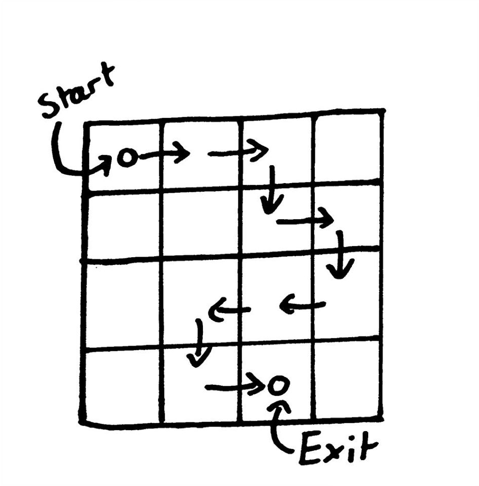
\includegraphics[width=\linewidth]{levelgen1.png}}
     \caption{Solution Path Generation}\label{Fig:Data1}
   \end{minipage}
   \begin {minipage}{0.49\textwidth}
     \frame{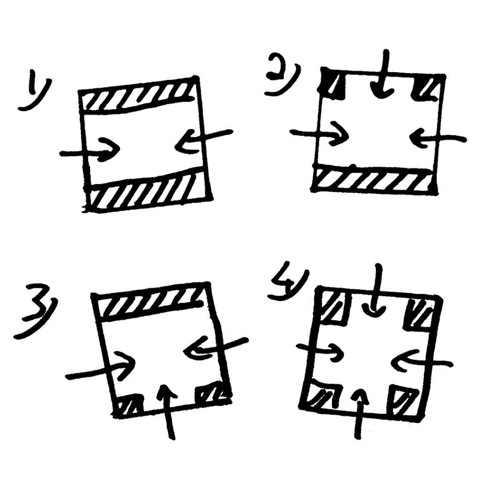
\includegraphics[width=\linewidth]{levelgen2.png}}
     \caption{Room Types}\label{Fig:Data2}
   \end{minipage}
\end{figure}

\subsection{Rooms}
Rooms are 16x16 grids of tiles, there are different rooms for the different exit types. Rooms are represented by \textit{CSV} text files an example of which can be seen in figure~\ref{Fig:Data3}. In the text files, different characters are used as identifiers for different tile types. For example \textit{G} represents a solid, walk-able surface, while \textit{T} represents a trap tile. Modifiers to the tiles, such as the radius of a light, can be added after the identifier. These can be easily swapped out of the game to create and test new levels.\\


\begin{figure}[!htb]\centering
   \begin{minipage}{0.49\textwidth}
     \frame{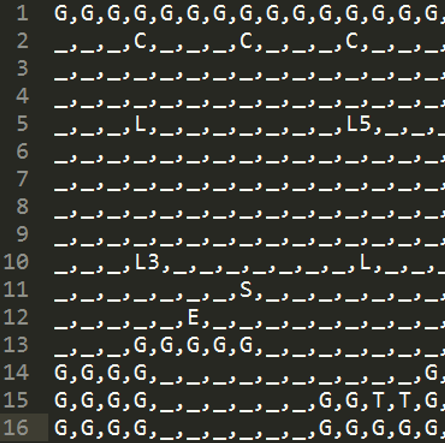
\includegraphics[width=\linewidth]{room.png}}
     \caption{Input text file}\label{Fig:Data3}
   \end{minipage}
   \begin {minipage}{0.49\textwidth}
     \frame{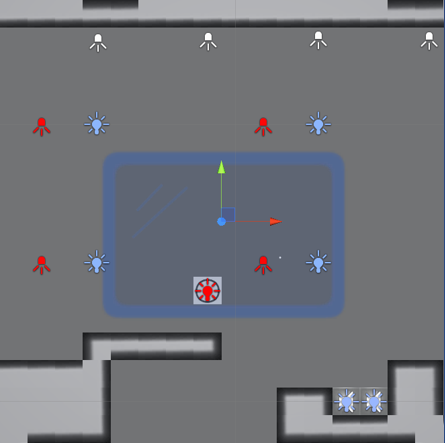
\includegraphics[width=\linewidth]{room1.png}}
     \caption{Unity Editor Output}\label{Fig:Data4}
   \end{minipage}
\end{figure}

\subsection{Lighting System}
To follow the theme, the game uses light to change the appearance of the level as the game progresses. We use three different sources of light in our game.\\

The first type of light is the spot light which is used for general illumination and ambience. The second type of light is the point light which is used to light specific areas. They are also used as spinning red alarm lights. These have three hard levels of dark, dim and bright which changes as components near them become reactivated.\\

The third method of lighting the scene is changing the ambient light level. As the player moves through the ship activating components the rooms towards the exit begin to light up. By varying the ambient light we can make dark areas harder to navigate and already explored areas brighter which helps highlighting where to go. \\

To emphasise the light effect on the level, normal mapped sprites are being used so as lights turn on and red alarm lights spin the level appears to react to it.
\subsection{Security System}
%Since the space ship's security system is malfunctioning, the game-play implemented in a way to have defence measures and show this unusual behaviour of security system using different components such as  electric traps, alarm and security droid/enemy.\\

The security system can be tripped when the player re-activates components of the ship. To turn it off the player needs to find another component of the ship and interface with it.\\

 When the ship enters an alarm state, the security droid begins chasing the player and electric traps are activated. The trap tiles kill the player with an electric bolt if they come in contact with them. The security droid can chase and attack the player by draining his energy. This forces the player to move fast to find the next ship component while dodging traps.

\subsection{Player Character}
The player controls the character directly as a traditional 2D platformer. The gameplay includes an energy system for the player. On re-activating a ship component, the player receives a portion of its energy back. The energy drains over time, encouraging the player to advance through the level.\\

The camera is dragged along by the player and moves in 3-dimensional space, the player can also hold the down button to move the camera down to check for traps lurking below drops. There are two lights attached to the player character. A spot light is used to light up the area in front of the player in dark rooms. A point light is used to draw attention to where the player is on screen and make him stand out.
\section{Team Organisation}
Scrum was used for the development of our game which is an iterative and incremental agile software development methodology for managing product development.\\

The team has used Jira for project management and Git for source control, synchronising progress across team and for maintaining stable and development branches.\\

The team created high level overview of tasks called Epics. The game different main components were divided into the following Epics: \textit{Level Generation}, \textit{GUI Creation}, \textit{Game Logic} and \textit{Player Character}.\\

These Epics were further broke down into smaller, more manageable stories. The project was divided into 4 sprints. Each sprint lasted for 2 weeks. At start of each sprint we had grooming sessions to estimate or re-estimate times for different stories and give more detailed descriptions of their implementations. Stories which were considered to be overly-complicated were broken down into smaller sub-task which could be more accurately estimated. Time estimation for different tasks was decided by using a voting system and then averaging everyone's estimates.\\

Team had regular stand-ups, an average of three times a week. Stand-ups were aimed to last for 10 minutes with any additional discussions happened in separate meeting outside this time. The team had a different scrum master for each sprint from each one of the team members.\\

Team prioritized the project stories by keeping Level generation and core game play features as high priority features and features secondary to a functional prototype such as a GUI for starting the game as low priority features. This was implemented for an organized way of development so that major game-play could be implemented on time keeping an account of time spent on other assignments of coursework. During the course of project, team learned more about Unity and skills/efficiency of different team members.

\section{Conclusion}
The team has implemented the core game mechanics as planned. Starting from the level generation with file handler to the lighting system, the alarm system and the enemy AI droid. There is also a rought user interface for starting and ending games and transitioning between levels.\\

\section{Future Work}

The way in which the game is created would allow for user created room files which would have been nice feature to explore if we had more time. A dedicated, visual, room editing tool was also discussed but the time-constraints of the project meant we had to stick with manually editing text files. 

\section{You Tube Link}

\section{Acknowledgements}
We would like to express our very great appreciation to Dr. John Dingliana for his valuable and constructive suggestions during the planning and development of this game. We would also like to acknowledge our friend Ting Zhang for her ideas for the asset creation and to work in collaboration with the whole team.  
\end{document}